\documentclass{beamer}
\usepackage[utf8]{inputenc}

\usetheme{Madrid}
\usecolortheme{default}
\usepackage{amsmath,amssymb,amsfonts,amsthm}
\usepackage{txfonts}
\usepackage{tkz-euclide}
\usepackage{listings}
\usepackage{adjustbox}
\usepackage{array}
\usepackage{tabularx}
\usepackage{gvv}
\usepackage{lmodern}
\usepackage{circuitikz}
\usepackage{tikz}
\usepackage{graphicx}

\setbeamertemplate{page number in head/foot}[totalframenumber]

\usepackage{tcolorbox}
\tcbuselibrary{minted,breakable,xparse,skins}



\definecolor{bg}{gray}{0.95}
\DeclareTCBListing{mintedbox}{O{}m!O{}}{%
	breakable=true,
	listing engine=minted,
	listing only,
	minted language=#2,
	minted style=default,
	minted options={%
		linenos,
		gobble=0,
		breaklines=true,
		breakafter=,,
		fontsize=\small,
		numbersep=8pt,
		#1},
	boxsep=0pt,
	left skip=0pt,
	right skip=0pt,
	left=25pt,
	right=0pt,
	top=3pt,
	bottom=3pt,
	arc=5pt,
	leftrule=0pt,
	rightrule=0pt,
	bottomrule=2pt,
	toprule=2pt,
	colback=bg,
	colframe=orange!70,
	enhanced,
	overlay={%
		\begin{tcbclipinterior}
			\fill[orange!20!white] (frame.south west) rectangle ([xshift=20pt]frame.north west);
	\end{tcbclipinterior}},
	#3,
}
\lstset{
	language=C,
	basicstyle=\ttfamily\small,
	keywordstyle=\color{blue},
	stringstyle=\color{orange},
	commentstyle=\color{green!60!black},
	numbers=left,
	numberstyle=\tiny\color{gray},
	breaklines=true,
	showstringspaces=false,
}
%------------------------------------------------------------
%This block of code defines the information to appear in the
%Title page
\title %optional
{2.5.4}
%\subtitle{A short story}

\author % (optional)
{Hema Havil - EE25BTECH11050}



\begin{document}
	
	\frame{\titlepage}
	\begin{frame}{Question}
		If $\vec{a}=2\hat{i}+y\hat{j}+\hat{k}$ and $\vec{b}=\hat{i}+2\hat{j}+3\hat{k}$ are two vectors for which the vector ($\vec{a}+\vec{b}$) is perpendicular to the vector ($\vec{a}-\vec{b}$), then find all the possible values of y.
	\end{frame}

	
\begin{frame}{Theoretical Solution}
         Let the given vectors be :\\ 
         \begin{align}
             \vec{a}=\myvec{2\\y\\1}  \vec{b}=\myvec{1\\2\\3}
         \end{align}
         Given that $\vec{a}+\vec{b}$ and $\vec{a}-\vec{b}$  are perpendicular, then \\
         \begin{align}
             \brak{\vec{a}+\vec{b}}^T\brak{\vec{a}-\vec{b}}=0
         \end{align}
         \begin{align}
             \vec{a}^T\vec{a}-\vec{b}^T\vec{b}=0
         \end{align}
         \begin{align}
             \vec{a}^T\vec{a}=\vec{b}^T\vec{b}
         \end{align}
\end{frame}
\begin{frame}{Theoretical Solution}
The values of $\vec{a}^T\vec{a}$ and $\vec{b}^T\vec{b}$ can be calculated by,
         \begin{align}
             \vec{a}^T\vec{a}=\myvec{2\;y\;1}\myvec{2\\y\\1}=4+y^2+1=5+y^2
         \end{align}
         \begin{align}
             \vec{b}^T\vec{b}=\myvec{1\;2\;3}\myvec{1\\2\\3}=1+4+9=14
         \end{align}
         From equation 0.4,\\
         \begin{align}
             5+y^2=14
         \end{align}
         \begin{align}
             y^2=9
         \end{align}
         \begin{align}
             y=\pm3
         \end{align}
         Therefore the values of y are 3 and -3
	\end{frame}
    
	
	\begin{frame}[fragile]
	\frametitle{C Code- Ploting the given vectors}
	
	\begin{lstlisting}

#include <stdio.h>
#include <math.h>
double matrix_multiply_transpose(const double u[3], const double v[3]) {
    double result = 0.0;
    for (int i = 0; i < 3; ++i)
        result += u[i] * v[i];  // Equivalent to u^T * v
    return result;
}

int solve_y_matrix_form(double* y1, double* y2) {
    double u1 = 2 + 1;     
    double u3 = 1 + 3;     
    double v1 = 2 - 1;     
    double v3 = 1 - 3;     
	\end{lstlisting}
\end{frame}
\begin{frame}[fragile]
\frametitle{C Code- Ploting the given vectors}
    \begin{lstlisting}
    double A = 1.0;   
    double B = 0.0;
    double C = -9.0;

    double discriminant = B*B - 4*A*C;
    if (discriminant < 0)
        return -1;

    double sqrt_disc = sqrt(discriminant);
    *y1 = (-B + sqrt_disc) / (2*A);
    *y2 = (-B - sqrt_disc) / (2*A);
    return 0;
}
    \end{lstlisting}
\end{frame}

\begin{frame}[fragile]
	\frametitle{Python Code using shared output}
	\begin{lstlisting}
		import ctypes
import numpy as np
import matplotlib.pyplot as plt

# Load C shared library
lib = ctypes.CDLL('./2.5.4.so')  # Change to .dll on Windows

# Define return and arg types
lib.solve_y_matrix_form.argtypes = [ctypes.POINTER(ctypes.c_double), ctypes.POINTER(ctypes.c_double)]
lib.solve_y_matrix_form.restype = ctypes.c_int

# Prepare output variables
y1 = ctypes.c_double()
y2 = ctypes.c_double()

# Call C function
res = lib.solve_y_matrix_form(ctypes.byref(y1), ctypes.byref(y2))

	\end{lstlisting}
\end{frame}
\begin{frame}[fragile]
	\frametitle{Python Code using shared output}
	\begin{lstlisting}	
     if res != 0:
    print("No real roots for y found.")
    exit()

y_values = [y1.value, y2.value]
print(f"Values of y computed using matrix multiplication in C: {y_values}")

# Plotting function
def plot_vectors_for_y(y_val):
    a = np.array([2, y_val, 1])
    b = np.array([1, 2, 3])
    a_plus_b = a + b
    a_minus_b = a - b
    origin = np.array([0, 0, 0])

    fig = plt.figure()
    ax = fig.add_subplot(111, projection='3d')

    
	\end{lstlisting}
\end{frame}
\begin{frame}[fragile]
	\frametitle{Python Code using shared output}
	\begin{lstlisting}
def draw(vec, color, label):
        ax.quiver(*origin, *vec, color=color, label=label, arrow_length_ratio=0.1)

    draw(a, 'red', 'a')
    draw(b, 'blue', 'b')
    draw(a_plus_b, 'green', 'a + b')
    draw(a_minus_b, 'purple', 'a - b')

    ax.set_xlim([-1, 6])
    ax.set_ylim([-4, 6])
    ax.set_zlim([-4, 6])
    ax.set_xlabel('X')
    ax.set_ylabel('Y')
    ax.set_zlabel('Z')
    

	\end{lstlisting}
\end{frame}
\begin{frame}[fragile]
\frametitle{Python Code using shared output}
\begin{lstlisting}
    ax.set_title(f'Vectors for y = {y_val}')
    ax.legend()
    plt.grid(True)
    plt.show()
for y in y_values:
    plot_vectors_for_y(y)
\end{lstlisting}
    
\end{frame}
\begin{frame}{Plot by python using shared output from c - 1}
	\begin{center}
	\begin{figure}[H]
		\centering
		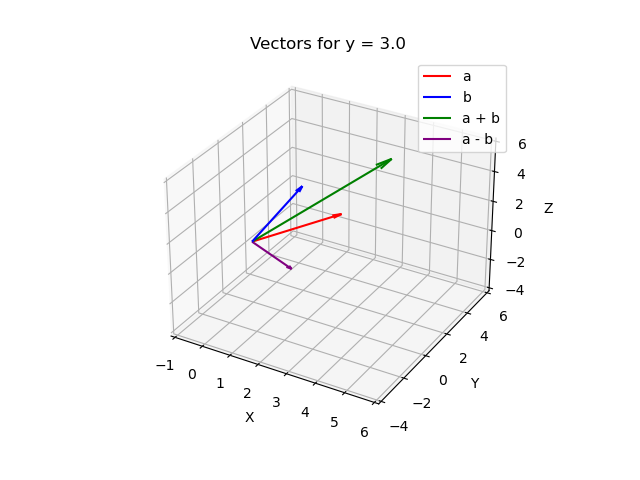
\includegraphics[width = 0.7\columnwidth]{figs/fig1.png}
		\caption{Plot of the vectors when y=3}
		\label{fig1}
	\end{figure}
	\end{center}
\end{frame}
\begin{frame}{Plot by python using shared output from c - 2}
\begin{figure}
    \centering
    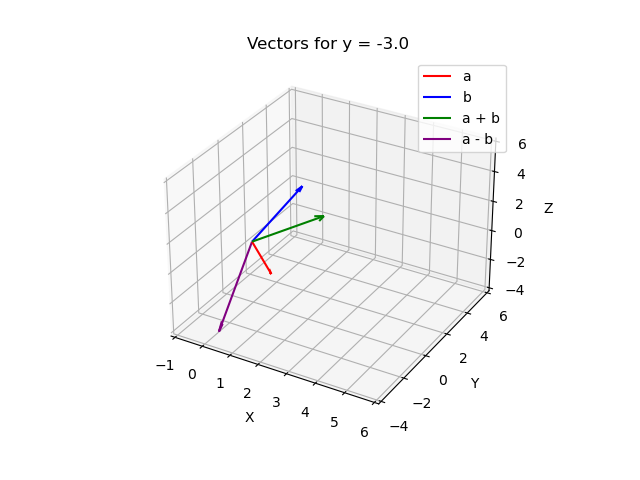
\includegraphics[width=0.7\columnwidth]{figs/fig2.png}
    \caption{Plot of the vectors when y=-3}
    \label{fig2}
\end{figure}
    
\end{frame}
\begin{frame}[fragile]
     \frametitle{Python code for the plot}
\begin{lstlisting}
    import numpy as np
import matplotlib.pyplot as plt

# Define vector b
b = np.array([1, 2, 3])

# Define a function for the condition (a+b) · (a-b) = 0
def find_y():
    # a = [2, y, 1]
    # Condition: (a + b) · (a - b) = 0
    # (2+1, y+2, 1+3) · (2-1, y-2, 1-3) = 0
    # Simplify: [3, y+2, 4] · [1, y-2, -2] = 0
    # Dot product: 3*1 + (y+2)*(y-2) + 4*(-2) = 0
    # 3 + (y^2 - 4) - 8 = 0 => y^2 - 9 = 0 => y = ±3
    y1 = 3
    y2 = -3
    return [y1, y2]





\end{lstlisting}
\end{frame}
\begin{frame}[fragile]
   \frametitle{Python code for the plot}
    \begin{lstlisting}
# Get possible y values
y_solutions = find_y()
print("Possible values of y:", y_solutions)

# Choose one y to plot
y = y_solutions[0]  # you can also try y_solutions[1]

# Define vectors a, a+b, a-b
a = np.array([2, y, 1])
a_plus_b = a + b
a_minus_b = a - b

# Plot vectors
fig = plt.figure()
ax = fig.add_subplot(111, projection='3d')
origin = np.array([0, 0, 0])
 \end{lstlisting}
\end{frame}
 \begin{frame}[fragile]
       \frametitle{Python code for plot}
       \begin{lstlisting}
      ax.quiver(*origin, *a_plus_b, color='r', label='a + b')
ax.quiver(*origin, *a_minus_b, color='b', label='a - b')

ax.set_xlim([0, 5])
ax.set_ylim([0, 5])
ax.set_zlim([0, 5])
ax.set_xlabel('X')
ax.set_ylabel('Y')
ax.set_zlabel('Z')
ax.legend()
plt.title(f'Vectors (a+b) and (a-b) for y={y}')
plt.show()
    \end{lstlisting}
 \end{frame}
 \begin{frame}{Plot of the vectors using python - 1}
     \begin{figure}
     \centering
     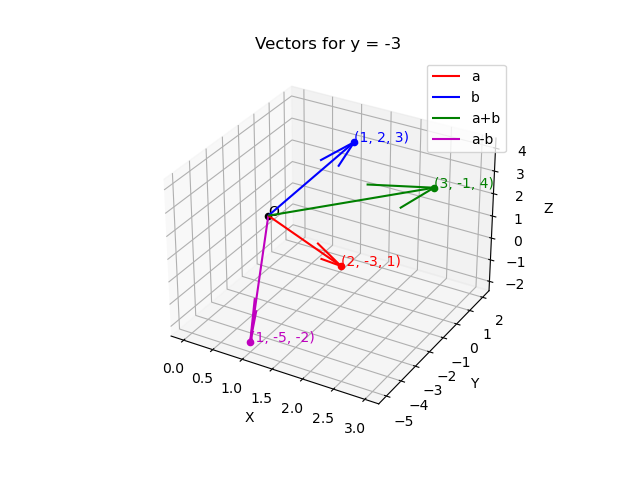
\includegraphics[width=0.7\linewidth]{figs/Fig1.png}
     \caption{Plot of the vectors when y=-3}
     \label{Fig2}
 \end{figure}
 \end{frame}
\begin{frame}{Plot of the vectors using python - 2}
    \begin{figure}
     \centering
     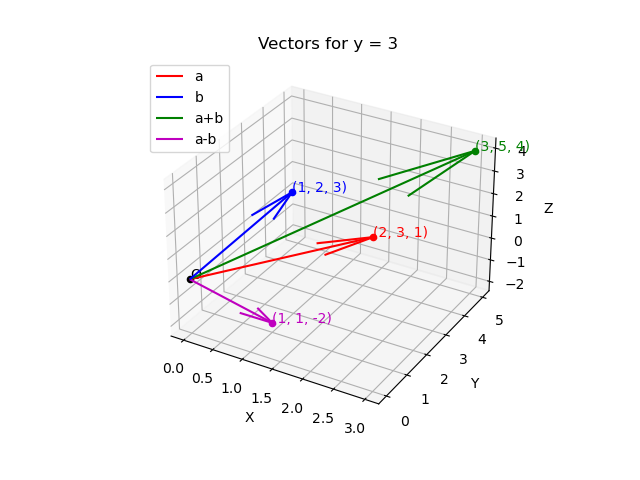
\includegraphics[width=0.7\linewidth]{figs/Fig2.png}
     \caption{Plot of the vectors when y=3}
     \label{fig:placeholder}
 \end{figure}
\end{frame} 
 
\end{document}